%!TEX root = index.tex

\chapter{Metodologia}

Será apresentado nesse capítulo a proposta de metodologia utilizada pelo autor para desenvolver o presente trabalho. Em primeira instância,  o objeto de estudo é apresentado, assim com as entidades associadas a ele. Posteriormente, são apresentadas as bases teóricas dos principais modelos analíticos utilizados na realização deste trabalho, de forma a esclarecer dúvidas quanto a sua utilização dentro do método apresentado. Por fim, a metodologia é esquematizada para ilustrar o alinhamento com os objetivos inicialmente definidos.

\section{Objeto de Estudo}

De forma a se aproximar de um dos principais nichos de seu interesse, a Samsung criou um programa de Relacionamento com Desenvolvedores, de forma a se aproximar de um dos grupos de profissionais que mais contribuem com a disseminação de novas tecnologias da Samsung. Esse programa é responsável por diversas ações, como o \textit{Developer Day}, que é um grande evento realizado uma vez por ano no Brasil e outros países da América Latina e visa promover as mais recentes tecnologias da marca, e também pelo Laboratório Ocean, objeto de estudo deste trabalho, que visa a aproximação da comunidade estudantil e de startups em formação.

O Laboratório Ocean é uma iniciativa da Samsung que tem como objetivo estimular desenvolvedores a criar soluções tecnológicas relacionadas aos produtos da marca coreana. A primeira sede do laboratório foi inaugurada em 2010 na Coréia do Sul, e a iniciativa foi replicada no Brasil há cerca de dois anos, com uma unidade em Manaus e outra em São Paulo. Ao passo que a unidade de Manaus foi estabelecida dentro da Universidade Estadual do Amazonas (UEA), a unidade de São Paulo encontrava-se até o fim de 2015 na Avenida Brigadeiro Faria Lima, uma das principais avenidas comerciais da cidade. Uma iniciativa recente movida por um ex-aluno, professores do departamento e o programa \enquote{Parceiros da Poli} trouxe através de conversas informais a ideia de trazer o laboratório para dentro da USP. Como o modelo intra universitário funcionou bem em Manaus, foi decidido replicar o modelo e sediar o laboratório dentro da Universidade, hospedado dentro do Departamento de Engenharia de Produção (PRO).

O Ocean fornece dois tipos de cursos, básicos e intensivos. Os cursos básicos são de curta duração (aproximadamente 3 horas), e os cursos intensivos em seu módulo atual duram 4 meses, utilizando o espaço toda noite de segunda à quinta-feira. O foco inicial dos cursos foi o desenvolvimento para dispositivos móveis, em especial apoiados no sistema operacional Android, inerente aos aparelhos da Samsung, como o Galaxy S7. Com o passar do tempo, os cursos começaram a seguir as tendências de \textit{hardware} do mercado e consequentemente da própria Samsung, como \textit{wearables}, \textit{smart} TVs, Internet das Coisas e Realidade Virtual. Mesmo assim, a área de dispositivos móveis ainda representa 80\% dos cursos oferecidos por eles.

Os cursos curtos possuem como principal objetivo despertar o interesse de desenvolvedores em relação aos produtos da Samsung. Portanto, os cursos trabalham de forma a mostrar todos os produtos de alta tecnologia da Samsung e capacitar desenvolvedores para que utilizem os seus dispositivos através do desenvolvimento de \textit{softwares}. Para tal, é disseminado tanto o funcionamento dos \textit{Software Development Kits} (SDKs) da Samsung e suas \textit{Application Program Interfaces} (APIs) para permitir o acesso ao \textit{hardware} dos seus dispositivos quanto o uso do Android para manipulação do software na linguagem nativa atual do sistema operacional utilizado por eles. Para a execução desses cursos, a Samsung trabalha juntamente com empresas terceiras especialistas no assunto para preparar o material a ser passado. Algumas vezes funcionários da própria Samsung dão o treinamento, e em alguns momentos houve até participação do corpo docente da Poli.

Os cursos intensivos são cursos de pré-aceleração de empresas, e têm o intuito de fomentar o empreendedorismo, apesar de manter a base de disseminar o conhecimento em cima de produtos da Samsung. A empresa acredita que no atual mercado, a diferenciação competitiva sobre o \textit{hardware} está ficando cada vez mais difícil, por isso as empresas estão buscando se diferenciar frente às outras em conteúdo. Dentro desse contexto, a Samsung visa auxiliar empresas a se desenvolverem e elas - em contrapartida - auxiliam a enriquecer os produtos da Samsung, seja através de novos produtos ou através de serviços.

Dessa forma, os cursos de pré-aceleração procuram fornecer conhecimento e experiência ao desenvolvimento de suas empresas, através de mentorias, bate-papo, palestras e avaliações. Como são cursos gratuitos, um dos principais desafios é manter o próprio engajamento das empresas, por isso o motivo de haver encontros 4 vezes por semana, com mentoria, criação e gestão do projeto proposto pelo programa, com checkpoints de avaliação das empresas ao longo do projeto. Tudo isso feito de forma \textit{gamificada} dentro do próprio modelo. A primeira parte do programa consiste na validação do modelo de negócio proposto pela empresa, e a segunda parte corresponde à prototipação e desenvolvimento de produto de fato. Atualmente contribuem com esse programa os profissionais da Samsung, funcionários terceiros, professores da USP, membros do NEU e empresas parceiras (Sebrae, FIESP, IBM, Amazon).

A infraestrutura do laboratório consiste em uma grande sala para até 80 pessoas, porém caso necessário portas retráteis permitem a sua divisão em duas salas separadas. Essa estrutura fica aberta das 08 às 22 horas de segunda a sexta feira, podendo ser utilizada livremente pela comunidade estudantil da universidade, cedendo computadores e acesso a Wi-Fi de alta velocidade. As mesmas salas são utilizadas para a realização dos cursos mencionados anteriormente.

Por se tratar de um acordo entre a Samsung e o PRO, é necessário que sejam feitas reuniões de alinhamento das necessidades e expectativas entre partes, que não estão sendo realizadas nesse primeiro momento pois o projeto ainda está no início e não há conflitos aparentes. Entretanto a universidade também tem planos para o laboratório e acredita que o mesmo terá um grande impacto dentro e fora da universidade. Segundo as palavras do professor Eduardo Zancul na inauguração do Ocean: “É uma frente de ensino, pesquisa e extensão. Ensino pois será um espaço para disciplinas do curso de engenharia de produção; Pesquisa porque materiais e a estrutura do laboratório serão utilizados pela comunidade acadêmica; Extensão pois muitos cursos serão abertos para a comunidade”. O laboratório se tornou uma parceria de cogestão entre universidade e empresa que tem como principal mérito a geração de valor derivada da sinergia entre academia e indústria. 

\section{Análises Utilizadas}

Ao longo do desenvolvimento do trabalho encontrou-se a oportunidade de utilizar modelos analíticos que atendessem a duas principais necessidades encontradas pelo autor: 

\begin{enumerate}
\item Análise de grandes quantidades de dados qualitativos
\item Condensação e simplificação de dados de diversas fontes em um mesmo modelo
\end{enumerate} 

De forma a resolver o primeiro problema, a Análise de Conteúdo é um ótimo modelo pois confere a base teórica para a categorização de informações obtidas a partir de dados qualitativos de forma eficiente. Em relação ao segundo, foi encontrado no modelo de Análise SWOT um método muito ilustrativo, com uma simplicidade correspondente ao nível de extração de informação desejado, atuando também como um guia de identificação de pontos de análise e de balizador para a montagem das entrevistas.

\subsection{Análise de Conteúdo}
\label{cha:analise_conteudo}

Após a realização de uma pesquisa com um alto número de pessoas, um dos principais obstáculos do pesquisador é analisar um grande volume de dados em tempo hábil e eficaz em relação à absorção de informação do conteúdo apresentado. Em muitos casos, a falta de conhecimento de métodos de análise leva os analistas a lerem e relerem individualmente todas as respostas de forma a obterem uma interpretação mais profunda dos dados, porém além de a eficiência ser muito baixa, não significa que a interpretação dos resultados terá uma eficácia alta. De forma a sintetizar as informações presentes em mensagens escritas, orais ou qualquer outro meio de comunicação de forma eficaz, a análise de conteúdo permite unir a camada lógica da linguística com a semântica da hermenêutica para fazer essa tarefa.

A análise de conteúdo é um dos métodos mais utilizados para a avaliação de estudos qualitativos e consiste em um conjunto de técnicas de análise de comunicações que permitem encontrar os principais significados de um grande volume de mensagens, através de métodos lógicos e semânticos. Ela tem como principal técnica a inferência, que consiste em produzir suposições subliminares sobre determinadas mensagens, embasando-se em características da mensagem como o contexto em que é produzida ou recebida. \cite{bardin}

Um elemento interessante dessa metodologia é a sua capacidade de gerar tanto análises quantitativas quanto qualitativas, e até modelos híbridos se for de interesse da pesquisa. Como ela trata principalmente do sentido dos elementos presentes no conteúdo das mensagens, ela pode sugerir tanto uma contagem de frases e palavras quanto uma consideração do estado emocional dos comunicadores, e obter inferências acima do número de ocorrências no primeiro caso e uma análise subjetiva do contexto do segundo caso.

O método de análise do modelo de \citeonline{bardin} pode ser simplificado em quatro principais etapas:

\begin{figure}[h]
\caption{Etapas da análise de conteúdo}
\centerline{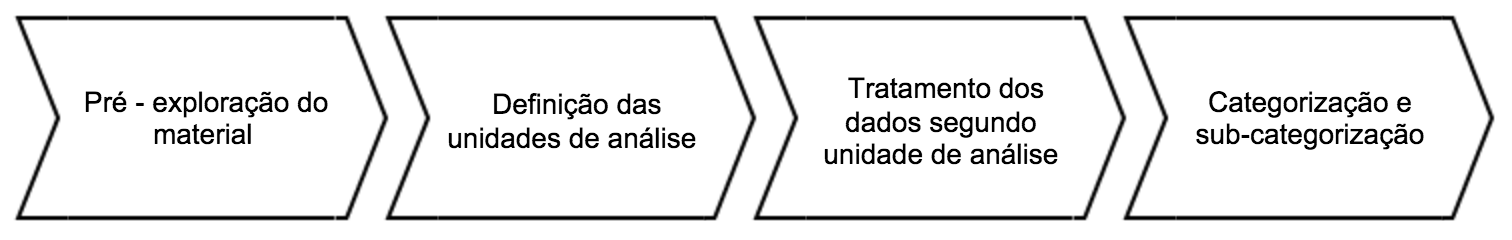
\includegraphics[scale=0.5]{img/fasesanalisedeconteudo}}
\label{fig:fasesanalisedeconteudo}
\caption* {Fonte: Simplificação do modelo \citeonline{bardin} realizada pelo autor}
\end{figure}

A fase inicial de pré-exploração tem como principal objetivo conhecer o contexto do material a ser analisado, retirar impressões e orientações para a próxima etapa. Um dos principais mecanismos dessa etapa é a leitura flutuante, que permite um primeiro contato com o conteúdo do \enquote{corpus de análise}, raso o suficiente para gerar a formulação de algumas hipóteses e não tomar tempo excessivo do analista. A leitura menos aderente permite a assimilação do \enquote{corpus de análise} de forma não-estruturada permitindo a transcendência da mensagem de forma explícita para visualizar pistas não inicialmente óbvias.

Em seguida, é necessário definir a unidade de análise a ser trabalhada, baseada no conteúdo do material avaliado. Essas unidades podem incluir palavras, frases, parágrafos, textos inteiros, de tal forma que possa ser feito algum tipo de análise utilizando-as. A partir das inferências obtidas na etapa anterior, é possível que já tenha sido visualizado que tipo de análise ou categorização poderia ser feito posteriormente, dependendo do tipo de dado analisado. Quando há uma grande repetição de informação devido a um escopo fechado de cada mensagem, é possível utilizar palavras ou frases como unidade de análise para uma posterior análise frequencial. Para os casos em que há uma diversidade maior de informação, a utilização de trechos maiores de texto permitem uma análise temática, a fins de categorização posterior.

Como pode se tratar de um grande volume de dados, é possível que haja a necessidade de um tratamento desses dados de forma a chegar em representações condensadas e explicativas. Para textos maiores, seria oportuno coletar somente as partes relevantes que explicam o conteúdo da própria mensagem passada. Já para palavras e frases, é possível que ocorram palavras sinônimas e frases com o mesmo conteúdo semântico, que tratadas dentro de um mesmo contexto facilitariam a sua categorização posterior. Dentro desse contexto, softwares simples de contagem de palavras até outros mais complexos baseados em algoritmos de \textit{Machine Learning} ganham um espaço de atuação muito grande nessa área, por agilizar esse tipo de tratamento.

Finalmente, através do tratamento desses dados, é possível segmentar as unidades de análise em categorias e em sub-categorias, se necessário. O nível de granularidade ou o gênero dessas categorias deve variar segundo os pontos que querem ser abordados na análise, entretanto recomenda-se fazer a categorização em um nível mais granular, para poder ser feita uma recategorização em níveis menos granulares posteriormente, se necessário.

\subsection{Análise SWOT}
\label{cha:analise_swot}

A análise SWOT é uma ferramenta utilizada para analisar o ambiente e o contexto em que uma empresa se encontra posicionada diante do mercado. O processo de utilização consiste basicamente em organizar características da empresa e do ambiente em que se encontra em quatro principais avaliações: Pontos Fortes (\textit{Strengths}), Pontos Fracos (\textit{Weaknesses}), Oportunidades (\textit{Opportunities}) e Ameaças (\textit{Threats}), conforme o quadro ilustrado abaixo. Essa modalidade de análise tem como principal vantagem a simplificação de uma estrutura complexa apresentada por uma organização, facilitando na tomada de decisões estratégicas.

\begin{figure}[H]
\caption{Quadro SWOT básico}
\centerline{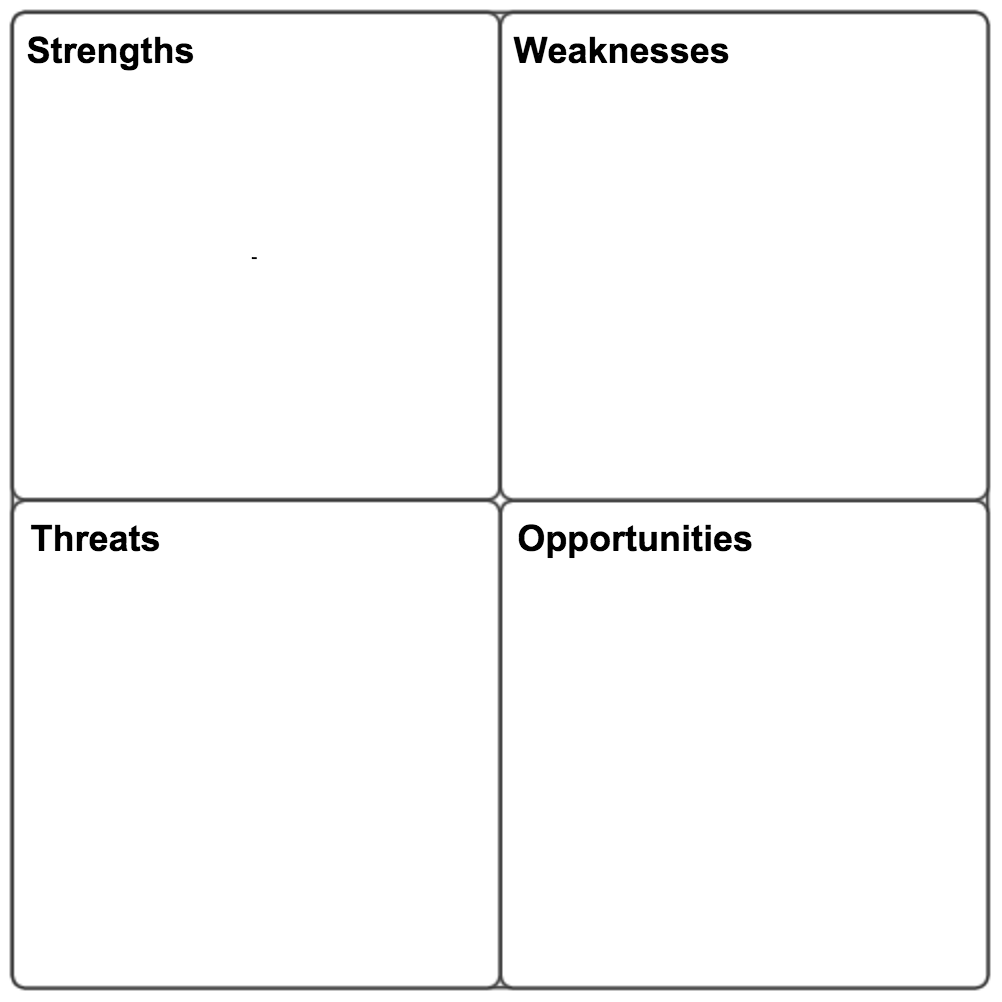
\includegraphics[scale=0.5]{img/detailedswot}}
\label{fig:detailedswot}
\caption* {Fonte: Quadro SWOT básico}
\end{figure}

\section{Método}

\label{chap:metodologia}

\begin{figure}[h]
\caption{Metodologia Utilizada no Trabalho}
\centerline{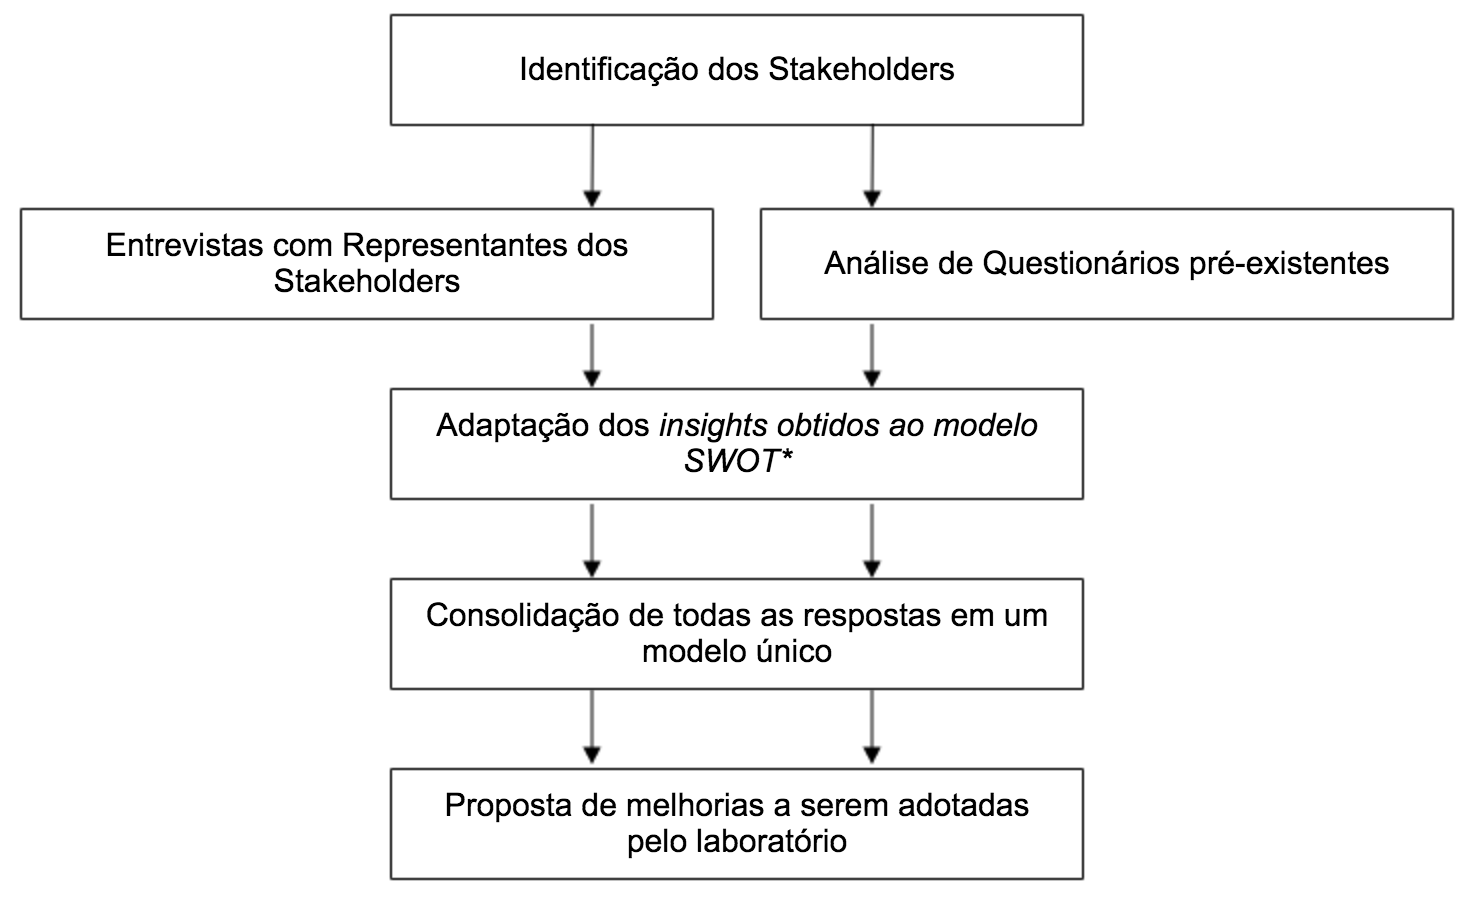
\includegraphics[scale=0.5]{img/metodologia}}
\label{fig:metodologia}
\caption* {Fonte: Elaborado pelo próprio autor}
\end{figure}

Após conversas iniciais com membros da Samsung e do PRO, foram definidos os stakeholders do projeto Ocean, juntamente com as pessoas-chave de cada. Foram realizadas entrevistas semi-estruturadas e gravadas, de forma a permitir a liberdade para serem feitas perguntas não presentes na estrutura inicial, e assim ter uma conversa guiada com o entrevistado como se não fosse uma entrevista formal. Antes de cada entrevista eram preparadas perguntas relacionadas ao mapeamento e percepção das interações do \textit{stakeholder} com o Ocean segundo a visão do entrevistador, e para todos os entrevistados era perguntado \enquote{se a pessoa teria alguma sugestão para a melhoria do Laboratório}.

Para análise de um \textit{stakeholder} em particular, representado pelo alunos dos cursos básicos do programa Ocean que serão apresentados nesse capítulo, o método de entrevistas foi considerado menos eficiente pelo alto número e rotatividade de alunos. Juntamente a este fato, a Samsung tinha uma necessidade de analisar questionários de \textit{feedback} respondidos nos últimos dois anos de cursos, que nunca haviam sido analisados diante das suas questões qualitativas, apenas das quantitativas. Dessa forma, foram unidas as necessidades de ambas as partes e foram aproveitados esses questionários - totalizando um total de 5280 respostas - para extrair as informações necessárias para este trabalho. O modelo de questionário aplicado encontra-se em anexo. No caso, foram analisadas somente as respostas das questões analíticas: \enquote{O que mais o motivou nesse curso?}, \enquote{O que você acha que pode ser melhorado?} e \enquote{Qual tema você gostaria que fosse abordado num próximo curso?}.

De forma a analisar e extrair informações desses questionários, o autor optou por desenvolver um software próprio (https://github.com/GabrielArakaki/wordAnalysis) para manipular esses dados via palavras-chave, pelos motivos elencados a seguir.

\begin{description}
\item [Volume de Dados] A quantidade de dados é grande o suficiente para dificultar - porém não inviabilizar - a leitura individual de cada uma das respostas. Acredita-se que mesmo que se optasse pela leitura individual, ela deveria ser acompanhada de uma categorização das respostas, o que a análise via repetição de palavras-chave também permite encontrar. Em contrapartida, os dados são suficientemente pequenos a ponto de não ser viável buscar alternativas  de \textit{Machine Learning} existentes para tratar esses dados, pois o volume não seria suficiente para treinar a inteligência artificial utilizada.

\item [Proposta do Estudo] Embora exista um campo muito grande de possibilidades de tratar e manipular os dados presentes, existe a necessidade de seguir com os objetivos inicias do presente estudo, que diz respeito ao estudo do projeto Ocean de forma holística, e não somente na questão do aprendizado transmitido através de seus cursos. O autor acredita que há espaço para análises mais sofisticadas - dignas de um trabalho dedicado somente a isso - que poderiam ser realizadas caso a Samsung encontre a necessidade de entender os cursistas nos mínimos detalhes.

\item [Manipulação de Dados] O uso de uma ferramenta própria dá ao autor a liberdade de trabalhar e iterar em cima dos dados de forma a otimizar a ferramenta para o próprio uso. Existem disponíveis ferramentas prontas de geração de nuvens de palavras, que possuem um intuito muito maior de apresentar um \enquote{choque visual} do que apresentar dados analíticos em si. A manipulação de dados permite que o autor encontre associações entre palavras ao observar os dados gerados pela ferramenta e trabalhar em cima da própria ferramenta para eliminar redundâncias ou dados inconsistentes.

\item [Desenvolvimento Ágil] O desenvolvimento ágil é um \textit{framework} de desenvolvimento de software que possui o intuito de permitir o desenvolvimento em um curto período de tempo com iterações feitas através da coleta de \textit{feedbacks} de forma rápida e sistemática. No caso deste trabalho, o autor não encontrou uma ferramenta que fornecesse customização e flexibilidade conforme suas necessidades, fazendo com que optasse por desenvolver um software próprio. Não obstante, é de satisfação do autor como desenvolvedor utilizar programação para resolver problemas reais.
 
\end{description}

Para consolidar a análise realizada para cada \textit{stakeholder}, foi utilizada uma adaptação do modelo SWOT para ilustrar as percepções obtidas de cada um. Ela difere do modelo original do SWOT por não se tratar de uma análise de negócio baseada em fatores de mercado e competitividade com outros \textit{players}, e sim em uma análise fria e absoluta de fatores básicos em um projeto: Pontos Fortes, Pontos Fracos, Oportunidades e Ameaças. Foi considerado que por ser um modelo simples e de fácil visualização, consolidaria as necessidades deste trabalho sem desvirtuar os objetivos propostos.

A partir dos resultados obtidos pela análise das respostas, trabalhou-se em cima da geração de propostas de melhoria.

\section{Identificação de Stakeholders do Laboratório}
\label{sec:identificacao_stakeholders}

A partir de conversas informais com os professores mais próximos ao projeto Ocean e com os próprios responsáveis da Samsung pelo laboratório, foi possível desenhar um mapa ilustrativo para os principais \textit{stakeholders}.

\begin{figure}[H]
\caption{Mapa de stakeholders do projeto Ocean}
\centerline{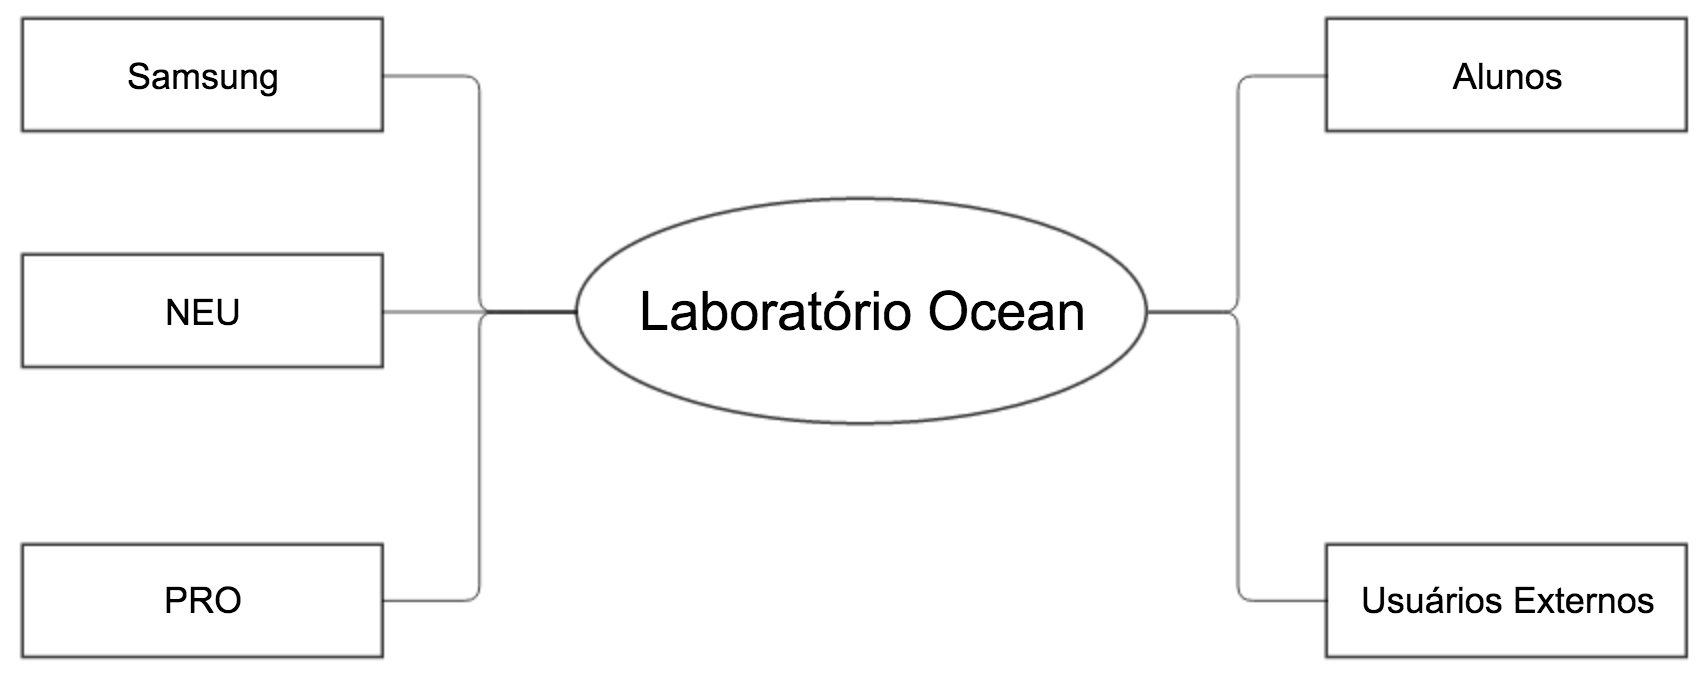
\includegraphics[scale=0.5]{img/stakeholders_v2}}
\label{fig:stakeholders}
\caption* {Fonte: Elaborado pelo próprio autor}
\end{figure}

Em um segundo momento foram definidos as principais fontes de dados para cada um dos \textit{stakeholders}, assim como os principais métodos de coleta, sendo definido o aproveitamento de questionários já respondidos pelos cursistas básicos e entrevistas para os demais.

\begin{figure}[H]
\caption{Pontos de contato dos \textit{stakeholders}}
\centerline{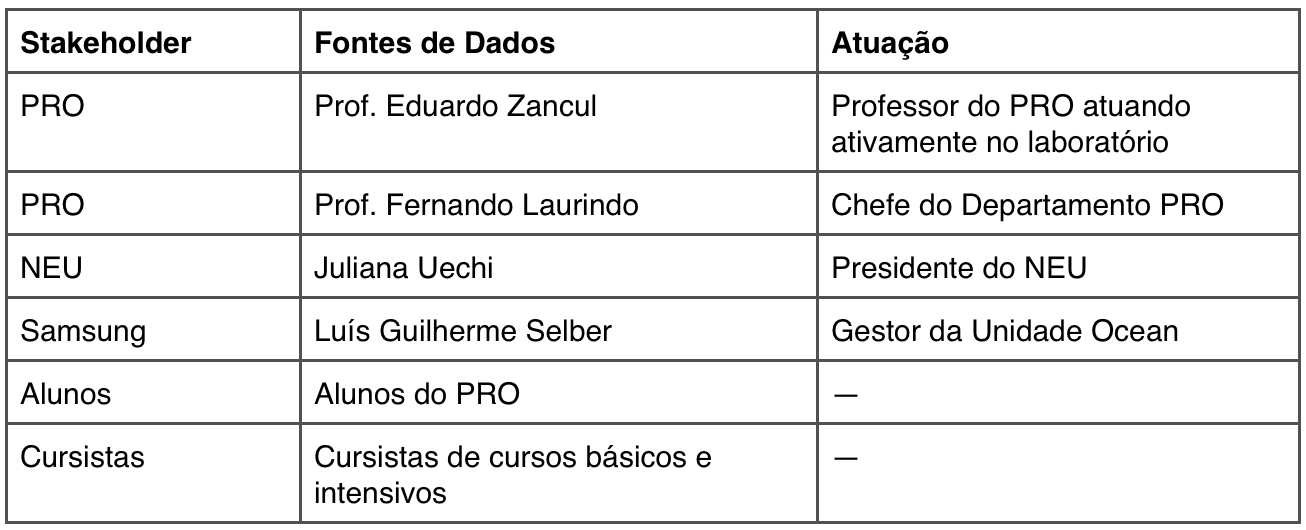
\includegraphics[scale=0.6]{img/stakeholderspoc}}
\label{fig:stakeholderspoc}
\caption* {Fonte: Elaborado pelo próprio autor}
\end{figure}


\subsection{PRO}
\label{sec:con_pro}

O Ocean faz parte de um grupo de quatro grandes projetos que o PRO acompanha atualmente, esquematizado pela Tabela \ref{tab:pilares_pro},  que também inclui as iniciativas Inovalab, a Fábrica Didática e o Núcleo de Empreendedorismo da USP.

\begin{table}[H]
\begin{center}
\caption{Pilares do PRO}
\label{tab:pilares_pro}
{\def\arraystretch{2}\tabcolsep=10pt
\begin{tabular}{>{\raggedright}p{0.2\linewidth}>{\raggedright\arraybackslash}p{0.2\linewidth}>{\raggedright\arraybackslash}p{0.2\linewidth}>{\raggedright\arraybackslash}p{0.2\linewidth}}
\hline
     & Objetivo Institucional & Participação do PRO & Em Atividade  \\ \hline
     Inovalab & Laboratório de Inovação & Gestão Ativa & Sim  \\
     Fábrica Didática & Apropriação de conceitos de fábricas para aplicação no ensino & Em Desenvolvimento & Não \\
     Ocean & Laboratório de Desenvolvimento de Software & Cogestão com a Samsung & Sim \\
	 Núcleo de Empreendedorismo da USP & Disseminação da cultura empreendedora & Cede espaço físico & Sim \\ \hline
\end{tabular}%
}
\caption* {Fonte: Elaborado pelo autor em conversa com professores do departamento}
\end{center}
\end{table}

O Inovalab é um laboratório que oferece recursos para realização de projetos de engenharia, como \textit{software}, \textit{hardware}, impressoras 3D e oficinas mecânicas. A infraestrutura do laboratório é utilizada para sediar o NEU, outro dos projetos que será discutido adiante. Já a Fábrica Didática é um projeto que consiste na produção de peças e produtos com a perspectiva de gerar pesquisa na área de fabricação e ensino para os alunos da engenharia de produção.

O que se pode ver em comum entre esses projetos e o Ocean é a proximidade da inovação e do empreendedorismo, pontos que o PRO considera essenciais para a tríade pesquisa, ensino e extensão. A Engenharia de Produção na Poli propicia um ambiente de aprendizado com disciplinas que já contribuem nessa área, como Projeto Integrado e Desenvolvimento de Produto, porém grande parte do aprendizado pode ser obtido através de atividades extra curriculares, propiciadas em parte por esses projetos. Um dos principais métodos de aprendizagem que a Poli incentiva nos alunos é o \textit{self-learning}, pois a área de Engenharia cobre uma variedade tão extensa de temas que o aluno que tiver interesse em se aprofundar em temas específicos deve buscar conhecimento por conta própria, sendo o principal papel da faculdade fornecer uma base sólida e uma estrutura para que ele possa adquirir conhecimento com facilidade.

\subsection{NEU}
\label{sec:con_neu}

O Núcleo de Empreendedorismo da USP é uma organização formada por alunos de graduação e pós-graduação, pesquisadores e professores que possuem a missão de promover a cultura de empreendedorismo dentro da Universidade. O NEU é aberto à toda comunidade da USP, já tendo recebido contribuições de diversas instituições da universidade, porém é formado atualmente principalmente por alunos da POLI e da FAU.

De forma similar ao estabelecimento do Ocean dentro do departamento do PRO, o NEU foi convidado a utilizar o espaço do InovaLab para sediar suas atividades. Atualmente o NEU trabalha com três principais pilares: inspiração, capacitação e conexão.

Inspiração diz respeito ao fomento ao empreendedorismo nos alunos para que eles se sintam impulsionados a participar do ecossistema de \textit{startups} ou até abrir as suas próprias. Portanto são feitos diversos convites aos diretores de diversas \textit{startups}, muitos com origens da própria USP, como Lean Survey, 99 Táxis e Squid, e estes podem explicar um pouco da sua trajetória e das emoções vividas graças aos seus empreendimentos. 

Capacitação é a frente do NEU de auxiliar ideias de alunos a se desenvolverem em produtos, para que assim sejam criadas novas empresas. A partir da rede de empresas que o NEU tem em seu leque de contatos, ele consegue encontrar mentorias para as empresas e acelerar o seu desenvolvimento. O principal programa dessa frente é o \textit{Startup Lab}, em que o NEU fornece material de apoio e mentoria através dos seus contatos com empresas, investidores e aceleradoras.

Conexão é representado principalmente pelo \textit{Startup Ship}, que é o canal do NEU destinado a alunos que querem estagiar em \textit{startups}. Através de sua rede de conexões ela facilita com que \textit{startups} e os alunos certos cheguem uns aos outros. Outro programa é o Pesquisas USP, que auxilia os alunos a se conectarem com pesquisas, e em contrapartida auxiliar pesquisadores a se conectarem com alunos ou empresas que possam auxiliar nos seus estudos. Nesse programa o NEU também auxilia startups a entrarem em contato com aceleradoras.

O NEU apresenta uma sinergia muito grande com o Ocean, pois ambos possuem muito interesse na fase de pré-aceleração de empresas, conseguindo exercer etapas distintas e complementares nesse processo. Durante os cursos intensivos do Ocean, o NEU se responsabiliza por trazer contatos de diferentes empresas para inspirar e fazer mentorias, ao passo que a Samsung trabalha fortemente na parte de capacitação e acompanhamento da evolução das empresas ao longo do programa.

Existe uma série de organismos dentro da universidade que fomentam a cultura de empreendedorismo, e como todos são gratuitos, existe uma colaboração muito grande para que os maiores beneficiados sejam as \textit{startups}, independente de  qual instituição que esteja contribuindo mais para a evolução da empresa.

\subsection{Alunos}
\label{sec:con_alunos}

A Engenharia de Produção é uma área que tem suas origens na engenharia mecânica, pois a formação de engenheiros no passado era voltada principalmente à capacitação técnica de produção de peças e produtos, sem um estudo aprofundado de como fabricá-los com eficiência. Os estudantes eram ensinados a desenhar um produto e desconstruí-lo em diversas peças que deveriam atuar conjuntamente para o funcionamento desejado. Encontrou-se então uma oportunidade de criar um novo ramo da Área Mecânica que se encarregaria de capacitar os alunos a aplicar conceitos de fábrica utilizados globalmente, como otimização das linhas de produção, controle da qualidade e controle da produção, não explorados anteriormente nos cursos de engenharia. Inicialmente voltado principalmente ao setor automotivo, a área de produção começou a ser expandida para poder aplicar os mesmos conceitos de fábrica para qualquer indústria, exigindo uma abstração dos principais conceitos, e inclusive a adoção de teorias de administração e gestão de projetos.

Atualmente, duas disciplinas eletivas do curso de Engenharia de Produção estão utilizando a infraestrutura do laboratório, Desenvolvimento Integrado de Produto e Criação de Negócios Tecnológicos, porém o laboratório cede seu espaço a disciplinas que necessitem dos seus recursos. Muitas das reclamações dos alunos em relação ao ensino atual diz respeito às aulas que são passadas utilizando tecnologias antigas, como retroprojetores. Embora o laboratório não esteja sendo usado pelas disciplinas obrigatórios, os alunos enxergam que a sua presença eleva o patamar de tecnologia de ensino a ser utilizado, o que no curto ou médio prazo pode abandonar as tecnologias antigas para adotar o maior uso de mídias digitais.

Além da questão das disciplinas, o laboratório é utilizado pelos alunos durante o período fora da aula, para a realização de trabalhos , tarefas ou para fixar o conteúdo que foi dado em aula. Como o laboratório fica aberto até as 22 horas, e na cultura da engenharia é bastante comum ficar até tarde estudando, alunos utilizam o laboratório praticamente o dia inteiro. Antes do laboratório era frequente os alunos irem estudar em outros departamentos como a Engenharia Civil, que possui várias mesas no seu saguão principal, e ficava aberta até tarde para os alunos de pós-graduação. Embora grande parte dos alunos traz o seu próprio \textit{notebook} para estudar, alguns utilizam os notebooks da própria Samsung e até um outro monitor para otimizar as suas tarefas.

A presença de um laboratório como este também ajuda a fomentar a cultura de empreendedorismo dentro da universidade, pois permite a capacitação dos alunos diante do desenvolvimento de produtos, base de criação de novas \textit{startups}. Segundo as pesquisas realizadas por \citeonline{entrepreneurship} com estudantes de graduação de engenharia, a experiência de empreendedorismo é observado de 4 maneiras, independentemente se eles desejam empreender ou não: 

\begin{enumerate}
\item Primeiro passo para o auto-aprendizado
\item Preparação para a vida no trabalho
\item Caminho para ser autônomo
\item Desenvolvimento de liderança e responsabilidade de um time
\end{enumerate}

Como esses pontos seguem na mesma direção dos objetivos da Poli e não agrada somente aqueles alunos que desejam ser empreendedores, o PRO pode continuar fomentando o empreendedorismo para que atinja todos os alunos. Entretanto, de forma a potencializar ainda mais os futuros empreendedores, é necessário entender o perfil daqueles alunos que desejam abrir o seu próprio negócio, como foi observado em diversas pesquisas como a realizada por \citeonline{empreendedorismo}, em que identifica o perfil de alunos que são atraídos pelo empreendedorismo:

\begin{itemize}
\item Propensão a assumir riscos
\item Proximidade a outros empreendedores no círculo próximo
\item Já possuem uma ideia desenvolvida para o empreendimento
\end{itemize}


\subsection{Cursistas}
\label{sec:con_cursistas}

Conforme explicado anteriormente, o Ocean trabalha com duas propostas de cursos, os cursos básicos e os cursos intensivos. O primeiro grupo corresponde à capacitação de desenvolvedores para que gerem conteúdo através de \textit{software} para dispositivos da Samsung, já o segundo é para pessoas que desejam empreender e possuem uma ideia inicial para ser desenvolvida. Embora exista uma gama de pessoas que seja usuária de ambos os cursos - os novos empreendedores têm muito interesse por programação - o público-alvo de cada um é diferente.

Os cursos básicos são desenhados para programadores ou aspirantes à programação. Embora existam diversos temas de cursos, o principal objetivo da Samsung consiste em capacitar os cursistas a explorarem todas as funcionalidades permitidas pelos \textit{hardwares} da Samsung. Para isso, são explorados o sistema operacional Android, os SDKs da Samsung, o sistema operacional Tizen, em suma tudo que possa contribuir para que o desenvolvedor possa gerar valor e conteúdo sem se preocupar em desenvolver um hardware específico. Portanto, é um curso de bastante interesse para iniciantes que desejam iniciar o aprendizado em programação, para desenvolvedores experientes que não tiveram muito contato com dispositivos móveis até para apaixonados pela Samsung que querem verificar na prática todo potencial permitido pelos seus dispositivos.

Segundo a 27\textsuperscript{a} Pesquisa de Anual do uso de TI, realizada pela Fundação Getúlio Vargas (FGV), o número de smartphones em uso no Brasil gira atualmente em torno de 168 milhões de dispositivos. \cite{tifgv}. Não obstante, além do alto número de smartphones, o Brasil também se mostra presente no mercado de outros dispositivos inteligentes, com previsão de movimentação de US\$4,1 bilhões no Brasil com IOT, segundo a assessoria de imprensa da IDC Brasil. \cite{idc}. Segundo a ONG Code.org, financiada por fundadores das maiores empresas de tecnologia do mundo como Mark Zuckerberg e Bill Gates, o número de empregos para programadores cresce exponencialmente, ao passo que o ensino de programação nas escolas não acompanha o mesmo ritmo, o que gerará uma falta de profissionais de TI em um futuro próximo. Juntamente a essa informação, o departamento de estatísticas de trabalho dos Estados Unidos (\textit{Bureau of Labor Statistics}) estima que o número de empregos para programadores fora dos EUA para trabalho remoto aumentará consideravelmente. \cite{bls}

É nesse cenário de alto crescimento do uso de novas tecnologias no Brasil que o mesmo se mostra como um grande mercado para produtos inerentes ao uso de dispositivos inteligentes, como aplicativos e games. Dentro desse contexto, jovens interessados pelo desenvolvimento desse mercado no país se interessam por propostas como a do Ocean para realizar diferentes cursos nessas áreas.
 
O segundo tipo de curso - cursos intensivos - foram feitos para incentivar ideias a se tornarem empresas, então é voltado para o nicho empreendedor. De acordo com o projeto \textit{Global Entrepreneurship Monitor}, que realiza pesquisas anuais sobre empreendedorismo no mundo, estima-se que em 2015, 52 milhões de brasileiros com idade entre 18 e 64 anos se envolveram na criação ou manutenção de algum negócio. Entre 2015 e 2014, houve um salto do total de empreendedores entre pessoas de 34,4\% para 39,9\% da população da faixa etária mencionada, principalmente devido ao surgimento de novas empresas. \cite{GEM}

Uma pequena parte dessas empresas é constituída de empresas com alto valor agregado e/ou com produtos de alta tecnologia, porém é visível o aumento da procura de pessoas que possuem ideias e buscam algum tipo de mentoria para desenvolvê-las a ponto de poder empreender. É nesse momento em que elas encontram o Ocean, onde podem utilizar de toda \textit{expertise} da Samsung para desenvolver um produto ou serviço de alta qualidade. Portanto não é necessário que os grupos já possuam uma empresa e um produto em funcionamento, até porque o programa desses cursos envolve questionar e validar hipóteses a respeito do próprio modelo de negócio da empresa, independente da maturidade da ideia. 

Os cursos intensivos são de uma extensão muito maior, e exigem uma intensidade muito grande dos cursistas, com reuniões de três horas de segunda à quinta-feira. Esse fator mostra a seriedade do programa em trabalhar com pessoas que mostrem um comprometimento acima da média, até porque muitos dos cursistas possuem emprego fixo e devem arranjar um tempo para se dedicar ao programa. Não obstante, além de ter esse acompanhamento quase diário nos dias úteis, são definidas metas semanais a serem cumpridas, para guiar as equipes no seu planejamento da semana. Toda essa intensidade tem o objetivo de deixar os alunos engajados ao longo do curso, que por ser gratuito e não exigir participação societária por parte da Samsung, pode facilmente ser abandonado se o aluno não observar o comprometimento da própria empresa.